\documentclass[twocolumn, 8pt]{article}
\usepackage[greek,francais]{babel}
\newcommand\tet{\textgreek{tetraf'armakos} }
\newcommand\IdC{I\textsuperscript{2}C }
\usepackage{eurosym}
\usepackage[T1]{fontenc}
\usepackage[utf8]{inputenc}
\usepackage[top=2cm, bottom=2cm, left=1cm, right=1cm]{geometry}
\setlength{\columnsep}{1cm}
\usepackage[usenames,dvipsnames]{color}
\usepackage{listings}
\lstset{language=C,
basicstyle=\ttfamily\small,
keywordstyle=\color{Blue}\bfseries,
identifierstyle=,
commentstyle=\color{Gray}, 
stringstyle=\color{BrickRed}\ttfamily,
morecomment=[l][\color{Green}]{\#},
showstringspaces=false,
tabsize=2,
numbers=left
}
\usepackage{graphicx}
\usepackage{amsmath,amssymb,amsfonts}
\usepackage{hyperref}

\title{Tutoriel de fabrication du \tet}
\author{Clément Javerzac-Galy \and{Denis Savoie}\\
	\texttt{\url{http://cansat2012.supop.fr}}
\and{Zubair Iftikhar}
}
\date{\today}

\begin{document}

\maketitle

\begin{abstract}
    \begin{bfseries}
	    \par \small Le projet \tet \footnote{pronouncez \textit{tetrapharmakos}} est un projet de Cansat réalisé par l'équipe des \textit{Proton-thérapeutes} de l'Institut d'Optique \textit{Graduate School} afin de participer au \textit{C'Space}, une compétition internationale co-organisée par Planète-Sciences et le CNES. 
	    \par \small Ce prototype de sonde spatiale embarque un module de mesure de l'indice de végétation fait-maison. Il enregistre en outre certains paramètres de vol à l'aide de divers capteurs (météorologiques et positionels).
    \par \small Nous espérons que toutes ces données mesurées permettront de caractériser les chances de présence de vie sur une exo-planète semblable à la Terre.
    \par \small Dans ce tutoriel, vous apprendrez à utiliser les différents composants que nous avons embarqués dans notre Cansat. Vous verrez comment tester le matériel, enregistrer les données mesurées sur une carte $\mu$SD et transférer des données à votre PC \textit{via} une liaison sans-fil.
     \end{bfseries}
\end{abstract}

\section{Matériel nécessaire}
Si vous souhaitez réaliser une copie exacte de notre projet (dont le coût total est d'environ 368\euro), il vous faudra:
\begin{enumerate}
	\item Contrôle et calculs:
		\begin{itemize}
			\item 2 x Micro-controlleurs Arduino Mini, 2 x 17\euro
			\item 1 adaptateur Arduino-Mini -- USB, 15\euro
		\end{itemize}
	\item Alimentation \footnote{Pour commencer, vous pouvez utiliser l'alimentation de la liaison USB entre votre Arduino et votre ordinateur.}
		\begin{itemize}
			\item 1 batterie 9V (NiMH), 13\euro
			\item 1 circuit d'adaptation de tension délivrant du 3,3V et du 5V, 5\euro
		\end{itemize}
	\item Stockage d'information
		\begin{itemize}
			\item 2 modules pour carte $\mu$SD, 2 x 13\euro
			\item 2 cartes $\mu$SD, 2 x 7\euro
		\end{itemize}
	\item Transfert de données sans-fil
		\begin{itemize}
			\item 2 modules XBee Pro, 2 x 36\euro 
			\item 1 \textit{dongle}-USB XBee, 21\euro
		\end{itemize}
	\item Capteurs
		\begin{itemize}
			\item 1 capteur d'humidité et température [RHT03], 15\euro
			\item 1 capteur de pression et température [BMP085], 18\euro
			\item 1 accéléromètre [ADXL345], 22\euro
			\item 1 module GPS [EM-406A], 29\euro 
			\item 2 caméras Jpeg [LinkSprite Jpeg TTL], 2 x 42\euro
		\end{itemize}
\end{enumerate}

\par Nous utilisons des composants en double car nous avons besoin de prendre deux photographies simultanées pour réaliser notre mesure de l'indice de végétation. Vous préfèrerez sans doute une Arduino Nano à une Mini, puisqu'elle est plus simple à programmer et à connecter à un ordinateur. Si vous voulez réduire les coûts et les contraintes techniques, voici la liste de composants à utiliser:
\begin{enumerate}
	\item Contrôle et calculs:
		\begin{itemize}
			\item 1 Micro-controlleurs Arduino Nano, 29\euro
		\end{itemize}
	\item Alimentation
		\begin{itemize}
			\item 1 batterie 9V (NiMH), 13\euro
			\item 1 circuit d'adaptation de tension délivrant du 3,3V et du 5V, 5\euro
		\end{itemize}
	\item Stockage d'information
		\begin{itemize}
			\item 1 modules pour carte $\mu$SD, 13\euro
			\item 1 cartes $\mu$SD, 7\euro
		\end{itemize}
	\item Transfert de données sans-fil
		\begin{itemize}
			\item 2 modules XBee, 2 x 26\euro 
			\item 1 \textit{dongle}-USB XBee, 21\euro
		\end{itemize}
	\item Capteurs
		\begin{itemize}
			\item 1 capteur d'humidité et température [RHT03], 15\euro
			\item 1 capteur de pression et température [BMP085], 18\euro
			\item 1 accéléromètre [ADXL345], 22\euro
			\item 1 module GPS [EM-406A], 29\euro 
			\item 1 caméras Jpeg [LinkSprite Jpeg TTL], 42\euro
		\end{itemize}
\end{enumerate}
Ce qui revient alors à 266\euro environ. Vous pouvez très bien adapter ce tutoriel à vos envies et choisir de faire une simple station météo (100\euro), ou un système de prise de photographies géolocalisées (138\euro).

\section{Assemblage et vérification du matériel}

\par Nous allons commencer par vérifier l'état de marche de chacun des composants. N'utilisez pas de pile au départ, l'alimentation se fera grâce à l'ordinateur. Par exemple si vous avez une Arduino Nano, il suffit de la connecter à votre ordinateur \textit{via} un câble USB (si vous utilisez une Arduino Mini, vous devez utiliser l'adaptateur Arduino FTDI USB-Série pour alimenter et programmer votre système).


\subsection{Le micro-contrôleur}
\par Pour savoir comment connecter votre Arduino à votre ordinateur pour la programmer, vous pouvez vous rendre sur le site officiel du fabricant: 
\begin{itemize}
	\item Arduino Mini: \url{http://arduino.cc/en/Guide/ArduinoMini}
	\item Arduino Nano: \url{http://arduino.cc/en/Guide/ArduinoNano}
\end{itemize}
\par Dans tous les cas, vous devez télécharger le logiciel de programmation Arduino sur \url{http://arduino.cc/en/Main/Software}. Utilisez le programme d'exemple \textsf{'Blink'} pour vérifier l'état de marche de votre micro-contrôleur.


\subsection{Le stockage sur carte $\mu$SD}
\par La plupart des applications nécessitent un enregistrement sur carte SD. Le prix de ces cartes mémoire Flash a beaucoup diminué, et on peut aujourd'hui facilement trouver une carte $\mu$SD de 2Go pour moins d'une dizaine d'euros. Il est recommandé d'utiliser des cartes de marque (j'avais une carte générique qui n'était pas reconnue, bien qu'elle soit bien formattée).

\par La figure \ref{SD} montre comment connecter le module de carte $\mu$SD à une Arduino Mini \footnote{Il faut savoir que les cartes SD doivent être alimentées en 3,3V, et que l'Arduino Mini fonctionne en 5V.}:

\begin{figure}[!h]
	\centering
	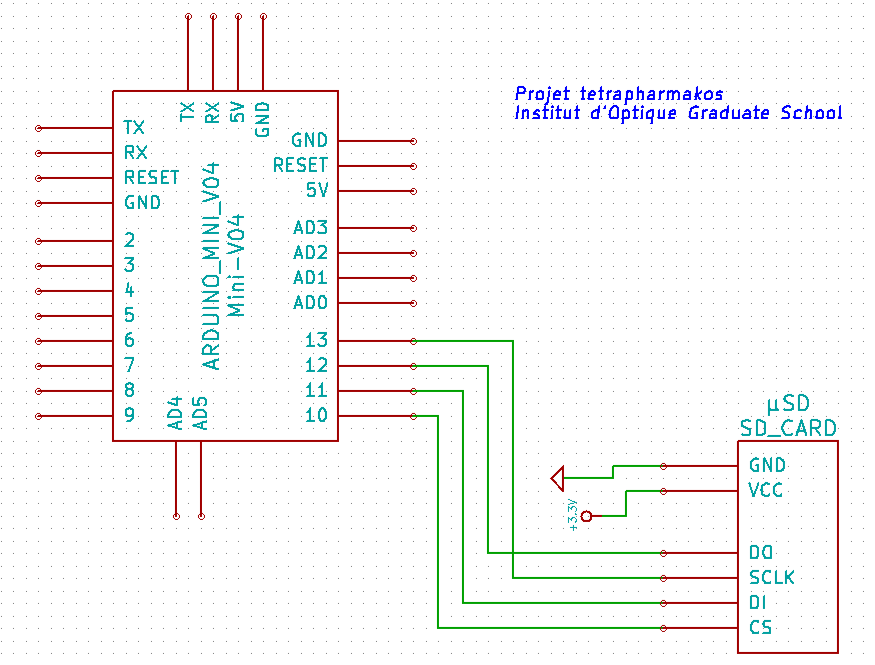
\includegraphics[scale=.25]{SD.png}
	\caption{Branchement d'une carte SD à une Arduino}
	\label{SD}
\end{figure}

\par Il faut alors utliser le programme d'exemple \textsf{'CardInfo'} du logiciel Arduino pour vérifier l'état de votre carte SD et de votre branchement.


\subsection{Les capteurs}
\par Notre Cansat devait remplir deux missions (sondage atmosphérique et mesure de l'indice de chlorophille). Pour la première, nous avions besoin d'un capteur d'humidité et d'un capteur de pression. Pour la seconde, nous avions besoin de deux caméra. L'accéléromètre et le module GPS étaient utilisés en vue de préparer une troisième mission: le atterissage maîtrisé sur une cible.

\subsubsection{Capteur d'humidité}
\par Le capteur d'humidité que nous avons utilisé est le \emph{RHT03}. Comme le reste des capteurs que nous avons utilisés, il est très simple d'emploi. La figure \ref{RHT03} montre comment le brancher \footnote{Il faut utiliser une résistance de tirage de 10k$\Omega$ entre la broche \no{}2 et l'alimentation +5V.}:

\begin{figure}[!h]
	\centering
	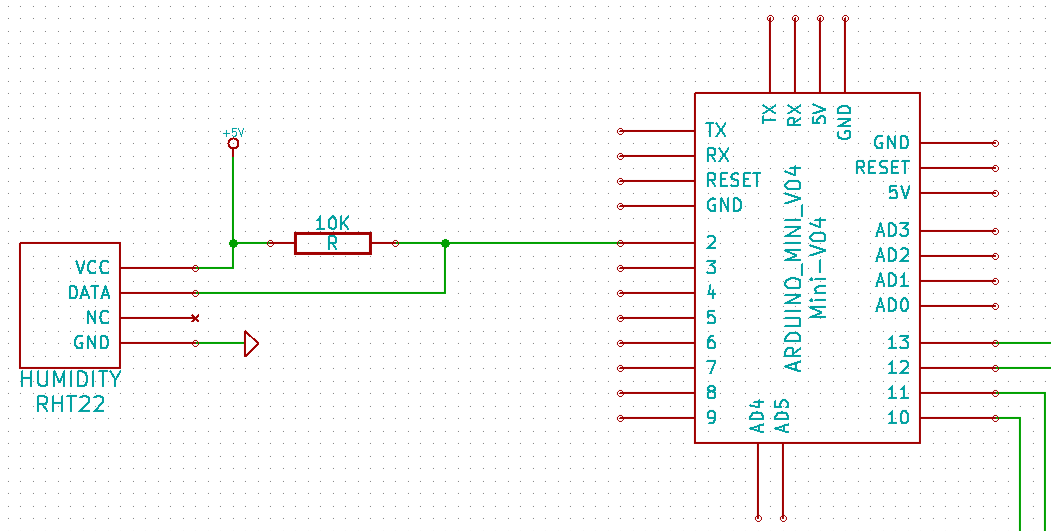
\includegraphics[scale=.2]{RHT03.png}
	\caption{Branchement du RHT03 à une Arduino}
	\label{RHT03}
\end{figure}

\par Il faut ensuite programmer votre micro-contrôleur pour envoyer les données du capteur sur le port Série de votre Arduino. Pour cela, téléchargez le programme \textsf{'DHTtester'} à l'adresse suivante: \url{https://github.com/thriller91/Cansat-SupOp/tree/master/sources/Arduino/DHT22/DHTtester}. Il faut télécharger les trois fichiers (\texttt{DHTtester.pde}, \texttt{DHT.cpp} et \texttt{DHT.h}), et les placer dans un même dossier appellé \textbf{DHTtester}.

\subsubsection{Capteur de pression}
\par Notre capteur de pression est le \emph{BMP085}. Il se connecte en \IdC. Comme le montre la figure \ref{BMP085}, il faut donc utiliser les broches analogiques \no{}4 et 5 de l'Arduino.

\begin{figure}[!h]
	\centering
	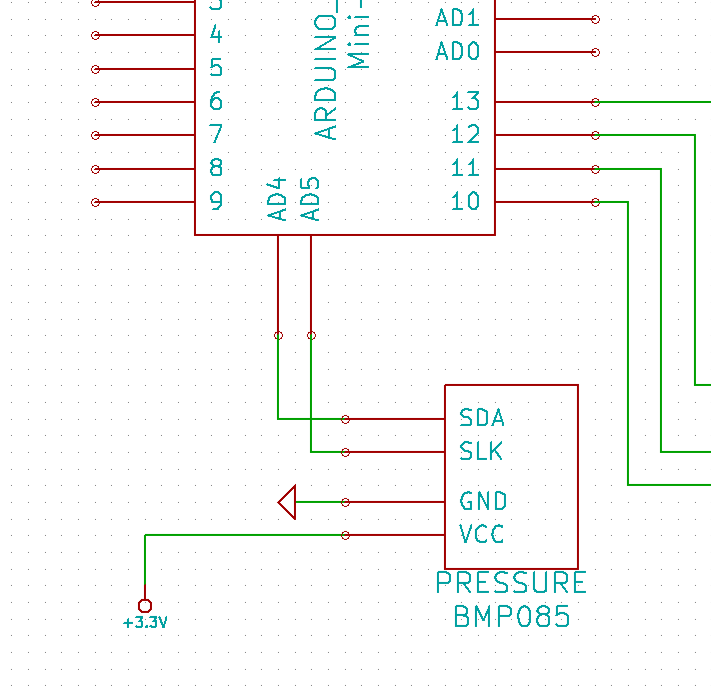
\includegraphics[scale=.2]{BMP085.png}
	\caption{Branchement du BMP085 à une Arduino}
	\label{BMP085}
\end{figure}

\par Le programme à télécharger pour essayer ce capteur est disponible à l'adresse suivante: \url{https://github.com/thriller91/Cansat-SupOp/tree/master/sources/Arduino/BMP085/BMP085tester}.

\subsubsection{Accéléromètre}
\par Nous avons utilisé un accéléromètre numérique, l'\emph{ADXL345}. Ce composant peut se connecter en \IdC ou en SPI (déjà utilisé par la carte SD). On peut connecter l'accéléromètre et le capteur de pression sur le même bus \IdC, mais comme nous avions 2 Arduino, nous avons utilisé une pour chaque capteur. Si vous voulez éviter d'utiliser une autre Arduino et que vous ne voulez pas placer ces deux composants sur le même bus, vous pouvez choisir d'utiliser un accéléromètre analogique (l'\emph{ADXL335} par exemple).

\par La figure \ref{ADXL345} montre comment brancher l'\emph{ADXL345} sur une Arduino en \IdC:

\begin{figure}[!h]
	\centering
	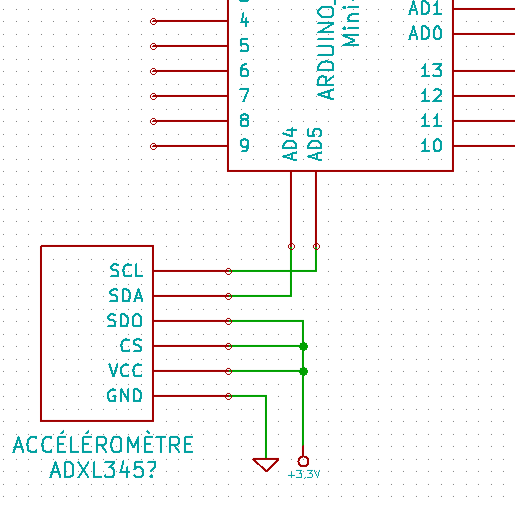
\includegraphics[scale=.25]{ADXL345.png}
	\caption{Branchement de l'ADXL345 en \IdC}
	\label{ADXL345}
\end{figure}


\end{document}
